
In this chapter, the method for generating synthetic images using Unity is outlined. The process begins with the creation of a virtual environment that simulates realistic maritime conditions, incorporating various elements such as water dynamics and weather conditions. Unity's rendering capabilities can generate a diverse set of images that serve as training data for computer vision models. By adjusting parameters such as lighting, camera angles and object placements, the dataset can reflect real world scenarios. 


\section{Creating the Virtual Environment}
Creating an virtual environment in Unity involves designing a scene that simulates real-world conditions. A scene in unity consist of two main components: a camera to capture the scene, and a 3D grid to define the spatial layout. Various objects and elements can be added to the 3D space, such as terrain, water, maritime objects and other 3D models. Additionally, animations can be added to simulate dynamic conditions such as water movement or rain which is important to create a realistic environment. Figure~\ref{fig:environment} shows an example of a scene created in Unity, featuring a water component and a dock harbor.

\begin{figure}[H]
    \centering
    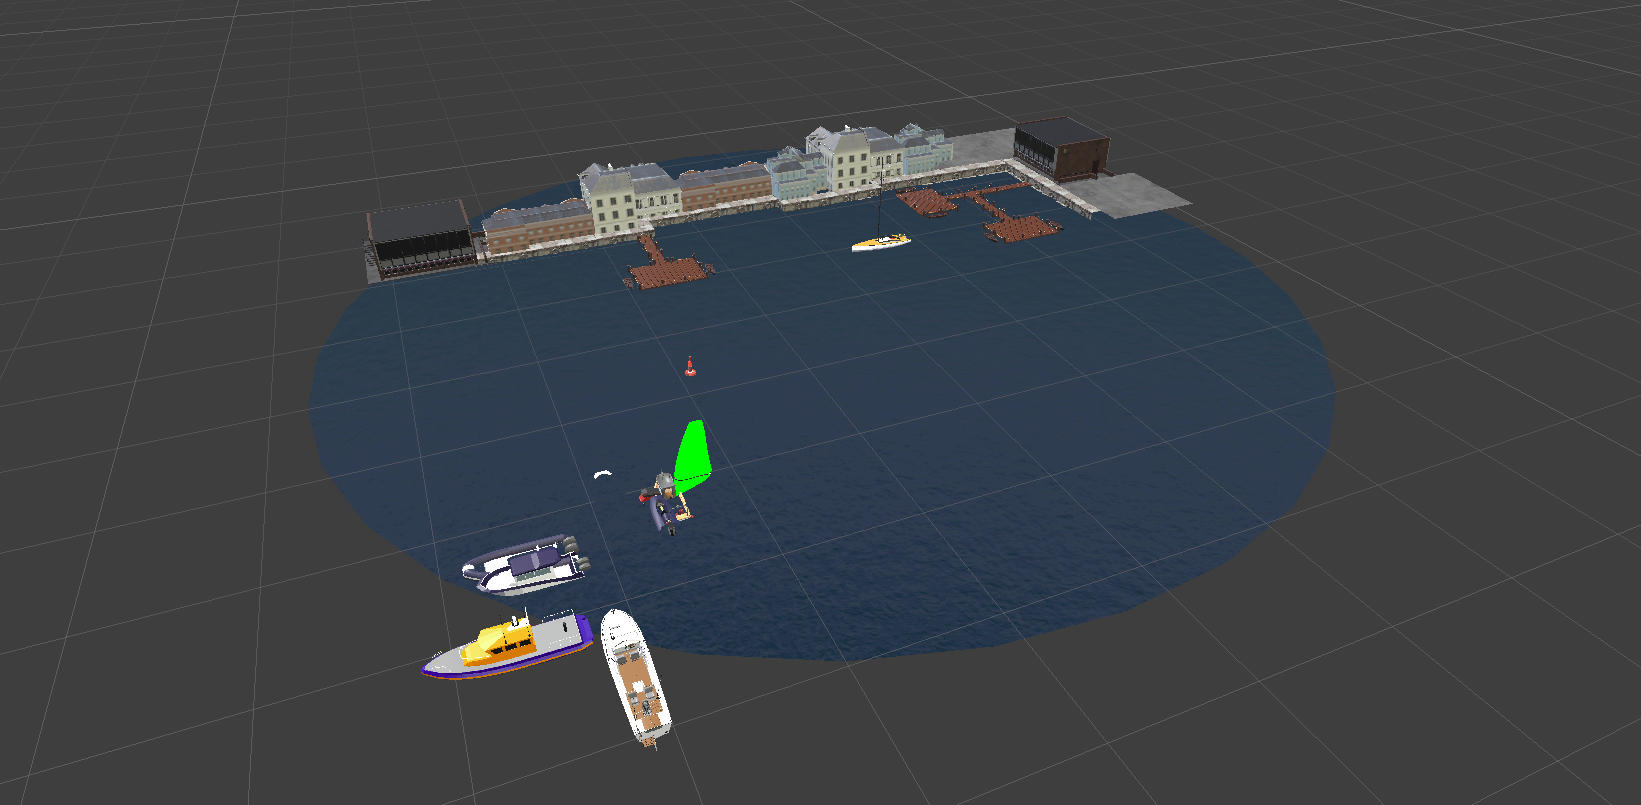
\includegraphics[width=0.9\textwidth]{Figures/method/environment2.png}
    \caption{The virtual environment in Unity.}
    \label{fig:environment}
    
\end{figure}
 
\subsection{Terrain}
Generating terrain in 3D space is a natural starting point for the virtual environment. The Unity \textit{Standard Asset Package} \cite{unity_standard_assets_installation} was used, providing a flat surface as a foundation. This package includes an environmental editor that allows users to manipulate the terrain and adjusting its shape by adding hills and valleys.

\subsection{Water}
The water surface was also imported from Unity's \textit{Standard Asset Package} \cite{unity_standard_assets_installation}, which offers a realistic water simulation. This asset provides a flexible water surface that users can adjust in both position and dimensions to fit the scene. The water is animated with small ripples to ensure it appears dynamic rather than as a still blue surface. However, the \textit{Standard Asset Package} does not support advanced water conditions, such as large waves. Given that this simulation focuses on object detection in a harbor environment with typically calm sea conditions, this limitation is not a significant concern.

\subsection{Weather}
To create a realistic environment, there is also important to generate a weather system. \textit{Rain Maker - 2D and 3D Rain Particle System for Unity} \cite{unity_rain_maker} was downloaded from Unity asset store and imported the prefab into Unity. This weather system allows for adjustments to rain and fog intensity. Additionally, the rain particles are animated to avoiding repetitive or identical images.

\section{Integrating 3D Models}
After creating the scene and environment, the next step is to integrate the 3D objects that will appear in the generated images. Since the focus is on harbor docking, the 3D models should represent common objects found in such environments. Common items include motorboats, sailboats, kayaks, buoys, windsurfers and other small watercraft. The process involves selecting the appropriate objects, sourcing models from various platforms, and integrating them into the scene.

\subsection{Sourcing 3D Models}
Several platforms offer free and paid 3D models. Free options were more limited in variety and quality, but they were enough to build a scene. Unity supports various file formats for importing 3D models, including 3DS, FBX, DAE, DXF and OBJ, which made it easier to work with assets from multiple sources. \\
\noindent The primary sources used to find models were:
\begin{itemize}
\item \textbf{Unity Asset Store}: A platform with many free and affordable assets and is also integrated with Unity platform \cite{UnityAssetStore}.
\item \textbf{CGTrader}: A marketplace that offers a wide selection of high-quality free 3D models \cite{cgtrader}.
\item \textbf{Sketchfab}: A community-driven platform for uploading, sharing and discovering 3D models \cite{sketchfab}.
\item \textbf{DNV}: Internal resources from DNV Wiki on DevAzure were also utilized. While it included some usable models suitable for harbor environments, some where large cargo ships, military frigates and RMS Queen Elizabeth which is not directly relevant \cite{dnv_wiki}.

\end{itemize}

\subsection{Adding 3D Models to the Environment}
Once the models were downloaded, they could be added to the Unity scene. The models were added to the project asset folder and then could be dragged into the scene in the Unity window. Firstly, a background featuring buildings and a dock was added to establish a harbor environment. Then, the different 3D objects were placed in front of the camera. The models where then positioned to be fully visible within the frame. The process involved trial and error to ensure that the scene looked natural and objects where visible in the frame.


\section{Implementation of Randomizers in Unity}
\label{section:Implementation of Randomizers in Unity}
After constructing the environment and importing all objects to be rendered, randomizers were implemented using the Unity Perception Package \cite{unity-perception2022}. Following Unity's perception guide \cite{unity-perception2022} and the YouTube tutorial \textit{Creating Randomized Synthetic Images with Unity3d Perception} \cite{secrets_of_apagayo_island_video}, the process involved the following steps:

\begin{itemize} \item \textbf{Create a Scenario}
The scenario object manages the randomization process and specifies the number of images to generate. It connects the randomizers to the environment, ensuring they work together to create a varied dataset. The scenario runs when the scene is played and coordinates all randomizers in a defined order \cite{borkman2021unityperceptiongeneratesynthetic}. The scenario can easily be added by dragging it from the perception package into the scene. For this project, the scenario was configured to generate 100 images, with parameters such as the number of frames and intervals set in Unity’s interface.

\item \textbf{Add Randomizers to the Scenario}: Randomizers introduce changes to specific aspects of the scene, such as camera positions, object colors and lighting conditions. Six randomizers were used: camera, sun angle, color, position, transformation and weather randomizers. Each randomizer was added to the scenario and configured with parameters to control the range of variation. Most parameters required trial and error to ensure a balanced dataset. Randomizers could also be linked to objects such as the camera, allowing it to interact with those elements during the randomization process.

\item \textbf{Apply Randomization Tags to 3D Objects}: When randomizers are added to a scenario, most are not connected to the objects. Different randomizers can be applied to various elements, such as foreground and background objects and some may affect multiple objects. To specify which objects to manipulate, a \texttt{randomization tag} component were added to each object. This tag directs the randomizer script to apply transformations to the tagged object.

\item \textbf{Label Objects for Ground Truth Data}: Labeling objects is essential for obtaining ground truth data. To do this, a \texttt{Labeling} component was added to each object and assigned a name. This component, which was a script included with the package, enabled labeling functionality. Next, the label name was added to both the BoundingBox and Semantic-SegmentationLabeler on the camera object. This ensured that Unity generated an RGB image for each frame along with a corresponding segmentation image.

\item \textbf{Generate Images}: Once the setup was complete, the scene was played to start the randomization process. Unity generated synthetic images with defined randomizers and parameters, creating a diverse dataset.
\end{itemize}


\section{Use of AI Tools in the Project}

AI tools such as ChatGPT and NotebookLM have become popular for generating content, answering questions and summarizing information. These tools were used throughout this project improving quality and efficiency. \\


\noindent For the literature study, academic articles were found using Google Scholar, a platform that helps finding peer-reviewed articles. Keywords such as "synthetic images," "Unity perception," "CV labeling," and "synthetic dataset performance" was used. Abstracts were then read to find the most interesting articles. NotebookLM was then used to summarize articles, answer specific questions about the content, and provide direct links to relevant sections of the documents.\\

\noindent AI-assisted tools were also used for coding to improve speed, and error resolution. GitHub Copilot, an AI model designed for programming, was used to generate code, fix errors and provide suggestions.\\

\noindent In addition, AI tools supported the writing process by enhancing grammar, correcting spelling, and improving clarity. ChatGPT contributed to making the text more polished and easier to read by offering feedback and suggestions for better phrasing.

% \section{generating ir images}

